\documentclass[hidelinks, 12pt]{article}



\makeatletter
\newcommand{\group}{B2-2}
\newcommand\footnoteref[1]{\protected@xdef\@thefnmark{\ref{#1}}\@footnotemark}
\makeatother
\usepackage{graphicx}
\usepackage{graphicx,hyperref,amsmath,bm,url}
\usepackage[numbers]{natbib}
\usepackage{microtype,todonotes}
\usepackage{a4}
\usepackage[compact,small]{titlesec}
\usepackage[utf8]{inputenc}
\clubpenalty = 10000
\widowpenalty = 10000
\usepackage[T1]{fontenc}
\graphicspath{ {../Billeder/} }
\usepackage{tikz}
\usetikzlibrary{calc}
\usetikzlibrary{shapes}
\usepackage[labelfont=bf]{caption}
\renewcommand{\figurename}{\textbf{Figur}}
\renewcommand{\contentsname}{Indholdfortegnelse}
\renewcommand{\refname}{Referencer}

\makeatletter
\newdimen\@myBoxHeight%
\newdimen\@myBoxDepth%
\newdimen\@myBoxWidth%
\newdimen\@myBoxSize%
\newcommand{\SquareBox}[2][]{%
    \settoheight{\@myBoxHeight}{#2}% Record height of box
    \settodepth{\@myBoxDepth}{#2}% Record depth of box
    \settowidth{\@myBoxWidth}{#2}% Record width of box
    \pgfmathsetlength{\@myBoxSize}{max(\@myBoxWidth,(\@myBoxHeight+\@myBoxDepth))}%
    \tikz \node [shape=rectangle, shape aspect=1,draw=red,inner sep=2\pgflinewidth, minimum size=\@myBoxSize,#1] {#2};%
}%
\makeatother
\newcommand*{\captionsource}[2]{%
  \caption[{#1}]{%
    #1%
    \\\hspace{\linewidth}%
    \textbf{Kilde:} #2%
  }%
}
\newcommand{\tabitem}{~~\llap{\textbullet}~~}
\begin{document}
	
	\title{Dagsorden}
	\author{Gruppe \group}
	\date{9. oktober 2015}
	\maketitle
	
	\noindent Vi har i gruppen lavet en brainstorm omkring emnet. Denne kan ses på figur \ref{fig:brainstorm}. Vi er desuden også kommet frem til et initierende problem som lyder:\\

	``Hvilke problemer står en skemalægger over for, under udarbejdelsen af skemaer i folkeskolen?''\\

	\noindent Vi har udarbejdet følgende spørgsmål som vi ønsker besvaret på gruppemødet.

	\begin{itemize}
		\item Hvor skal vi beskrive den teori vi bruger til programmet (genetiske algoritmer)?
		\item Hvor lang forventer I at rapporten skal være?
	\end{itemize}

	\noindent Vi ønsker på mødet at:
	\begin{itemize}
		\item få svar på spørgsmålene nævnt ovenfor
		\item snakke om en vejlederkontrakt
		\item snakke om jeres interesser, og hvordan I mener at I hver især bedst kan vejlede gruppen 
		\item få planlagt fremtidige møder
	\end{itemize}
	
	\begin{figure}[t!]
	\centering
		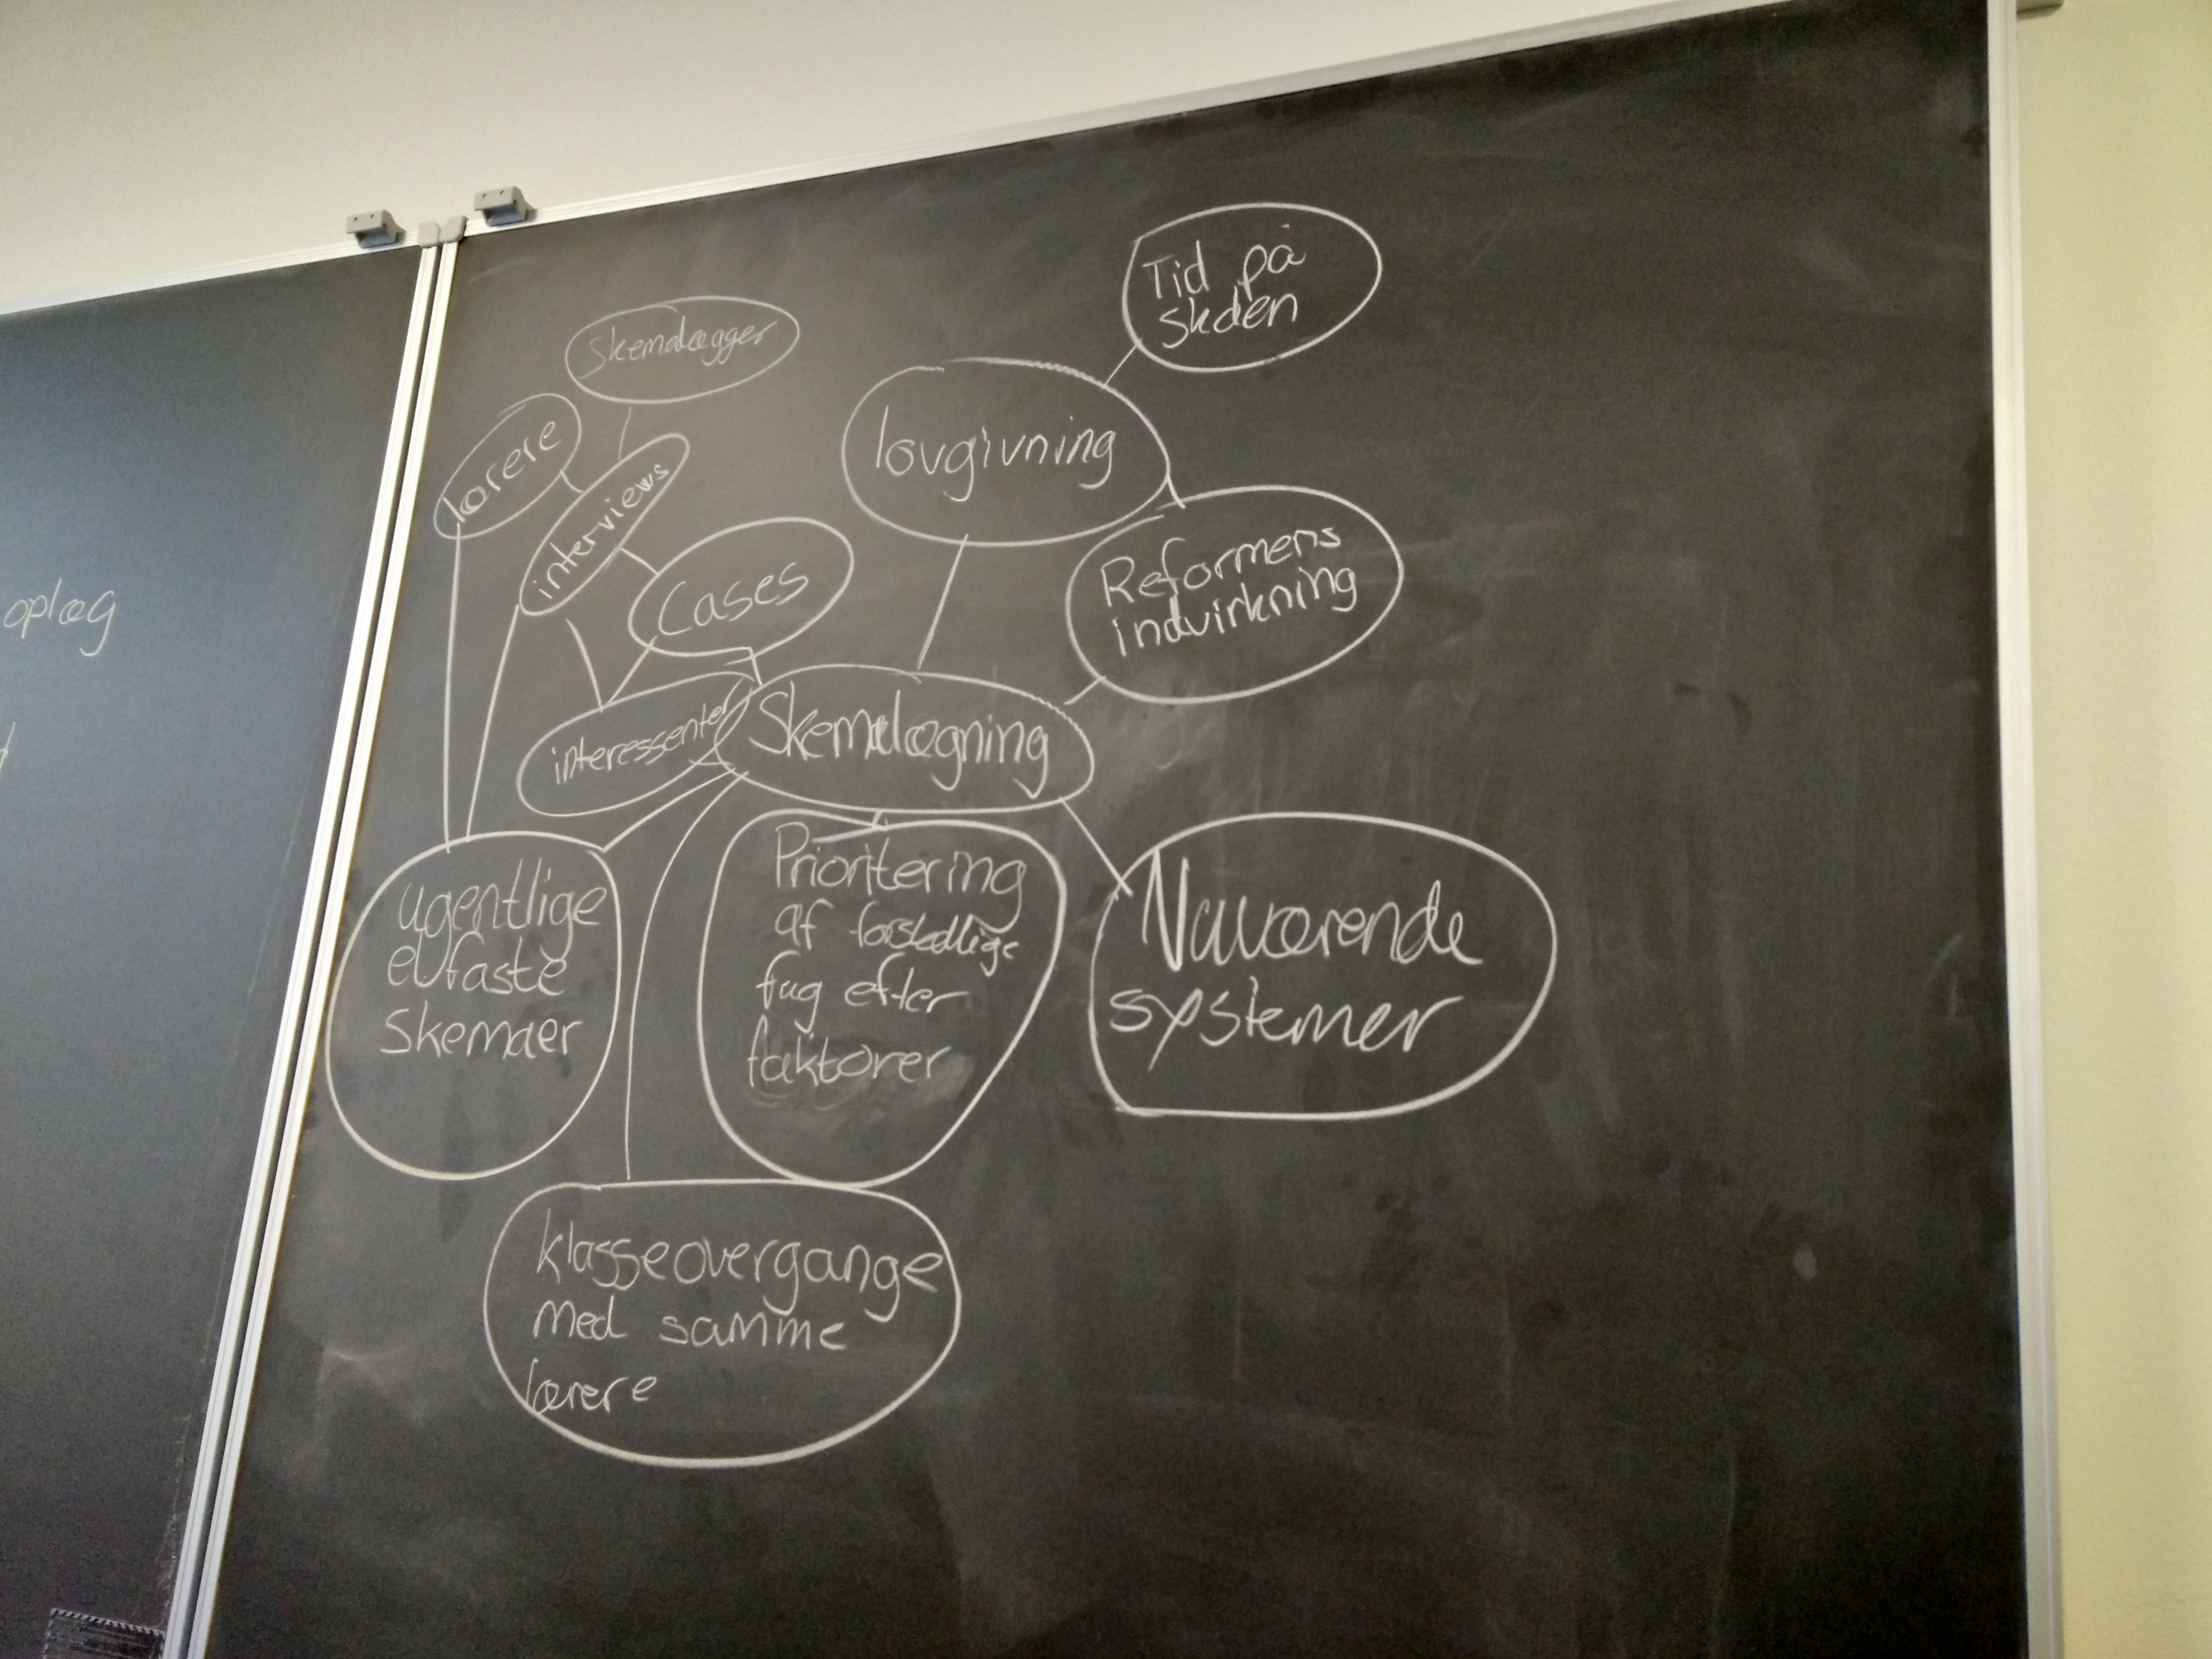
\includegraphics[width=\textwidth]{brainstorm}
		\caption{Brainstorm}
		\label{fig:brainstorm}

	\end{figure}
\end{document}